\documentclass[10pt]{article}
\usepackage[utf8]{inputenc}
\usepackage{amsmath,setspace,geometry}
\usepackage{amsfonts}
\usepackage[shortlabels]{enumitem}
%\usepackage[dvipdfmx]{hyperref,graphicx}
\usepackage{graphicx}
\usepackage{bbm}

\usepackage[colorlinks,citecolor=purple,urlcolor=blue,bookmarks=false,hypertexnames=true]{hyperref}
\usepackage[]{natbib} 
\bibpunct[:]{(}{)}{,}{a}{}{,}
\geometry{left = 1.0in,right = 1.0in,top = 1.0in,bottom = 1.0in}
%\onehalfspacing
% \usepackage{setspace}
\doublespacing
%\renewcommand{\baselinestretch}{0.3}
\usepackage[english]{babel}
\usepackage{float}
\usepackage{subfig}
\usepackage{booktabs}
\usepackage{pdfpages}
\usepackage{threeparttable}
\usepackage{lscape}
%\setstretch{1.2}
\newtheorem{assumption}{Assumption}
\newtheorem{definition}{Definition}
\newtheorem{example}{Example}
\newtheorem{lemma}{Lemma}

\title{Unified Merger List in the Container Shipping Industry between 1966 and 2022: Transition of Importance of Firms' Age, Tonnage Capacity, and Geographical Proximity on Merger Decision}
\author{Suguru Otani\thanks{Department of Economics, Rice University. Email: so19@rice.edu}\quad  Takuma Matsuda\thanks{Faculty of Commerce, Takushoku University. Email: tmatsuda@ner.takushoku-u.ac.jp}}
\date{
First version: XXX\\
Current version: \today
}

\begin{document}

\maketitle

\begin{abstract}
We construct a novel unified list of mergers in the global container shipping industry between 1966  (the beginning of the industry) and 2022. Combining the list with proprietary data, we construct a structural matching model \citep{fox2018qe} to describe the historical transition of the importance of a firm's age, size, and geographical proximity on merger decisions. 
We find that, as a positive factor, a firm's size is more important than a firm's age by seven to nine times as a merger incentive between 1991 and 2005.
On the other hand, between 2006 and 2022, as a negative factor, a firm's size is more important than a firm's age by 1.4 times, that is, the firm's size works as a disincentive.
We also find that the distance between buyer and seller firms works as a disincentive for the whole period, but the importance level has decreased to economically zero in recent years. 
In counterfactual simulations, we find that the prohibition of mergers between firms in the same country affects not only the number of permitted mergers in different countries but also the merger configuration, that is, buyer-seller-match pairs.
\end{abstract} 

\vspace{0.1in}
\noindent\textbf{Keywords:} container shipping industry; exemption agreement;  merger; matching 
\vspace{0in}


\section{Introduction}

Container shipping is a crucial component of global trade that has revolutionized the world. 
According to IHS Markit and Descartes Datamyne, container shipping accounts for $45.4 \%$ of amount-based imports to the U.S., $21.3 \%$ of amount-based exports from the U.S., and $10.12 \%$ of quantity-based world trade are shipped in 2021. 
Additionally, the container shipping industry offers a fascinating opportunity to explore not only industry dynamics such as entry, exit, and investment \citep{otani2023industry}, but also merger waves since the industry began global shipping operations in 1966. 
Despite its significance, like route-year-level prices and quantities dataset constructed by \cite{matsuda2022unified}, there is a lack of a unified dataset for the mergers in the container shipping industry, particularly for the years 1966 to 1990, which limits quantitative research evaluating mergers. 
This study provides a unified list of all realized mergers in the container shipping industry between 1966 and 2022.

Using our new merger list, we first illustrate the merger waves between 1966 and 2022 in the global container shipping industry and compare them with the transitions of prices and quantities constructed by \cite{matsuda2022unified}. 
We find that merger waves occurred after the enactment of the Shipping Act of 1984, that is, cartel breakdown, and significant merger waves were observed after 2005, corresponding to the exponentially growing quantity trend under competitive prices.
This suggests that we divide the industry history into three \textit{regimes}, 1966-1990, 1991-2005, and 2006-2022 following the corresponding data.
Second, combining our merger list with proprietary ship-level data, we provide the merger patterns that mergers are likely to involve relatively younger and smaller firms in more distant countries in recent years. 
\textcolor{blue}{The data patterns are consistent with institutional evidence that XXX. For example, XXX.}

The merger pattern yields several important insights into the merger waves in the global container shipping industry. 
However, there are several potential reasons for observing this pattern. 
For example, firms might put greater importance on a firm's size to increase tonnage shares within the market in the decision to buy firms in recent years rather than the period between 1966 and 1990. 
Alternatively, firms might put greater importance on geographical proximity to achieve the dominant position at the local country level. 
To disentangle these explanations and gain much more detailed insights into the different channels in a sophisticated way, we construct a structural model to quantify the relative importance of a firm's age, size, and geographical proximity by applying a novel approach, that is, matching maximum score estimator \cite{fox2018qe}. 

Our estimation results indicate that assortativeness of both size and geographical proximity contributes to merger incentives or disincentives. 
First, the assortativeness of the firm's size changes from negative between 1991 and 2005 to positive between 2006 and 2022. 
This implies that, between 1991 and 2005, as a positive factor, a firm's size is more important than a firm's age by seven to nine times in merger decisions, that is, a firm's size works as a merger incentive.
On the other hand, between 2006 and 2022, as a negative factor, a firm's size is more important than a firm's age by 1.4 times, that is, a firm's size works as a merger disincentive.
Second, we find that geographical distance works as a merger disincentive for the whole period, but the importance level relative to a firm's age has decreased to economically zero in recent years. 
This implies that merger incentives to achieve the dominant position at the local country level decrease.

Finally, we exercise a counterfactual simulation given the estimated parameters. 
We investigate the effect of the prohibition of mergers between firms in the same country on matching outcomes. This type of blocking merger is the most controversial topic in competition policies. 
For example, on June 21, 2017, South Africa's Competition Commission issued a statement stating that it "forbade" the integration of the container business by the three shipping lines of NYK, MOL, and KLINE. 
The commission cited concerns about market consolidation by domestic companies and cartel issues involving these companies in the car carrier business.
The country's competition court finally approved the integration on January 17, 2018, but this could impact the planned launch of the integrated container company, Ocean Network Express.
In counterfactual simulations, we find that the prohibition of mergers between firms in the same country affects not only the number of permitted mergers in different countries but also the merger configuration, that is, buyer-seller-match pairs.


\subsection{Related literature}

This paper contributes to three strands of the literature, namely, empirical transferable utility (TU) matching, endogenous merger analysis, and recent industrial policy and antitrust studies in the shipping industry.

First, this paper contributes to the literature on empirical TU matching. 
The most related econometric model is \cite{fox2018qe}, whose model has been applied to other empirical topics such as banking merger \citep{akkus2015ms,chen2013ijio}, faculty room allocation \citep{baccara2012aer}, executive and firm matching \citep{pan2017determinants}, and buyer and seller relationships in the broadcast television industry \citep{stahl2016aer}. 
These papers have applied the matching maximum score estimator proposed by \cite{fox2010qe,fox2018qe} to two-sided many-to-many and one-to-one matching in a TU matching environment. 
We apply the approach to merger waves in the global container shipping industry from its inception by dividing the history into three regimes based on institutional knowledge and data period.

Second, this paper contributes to the literature on endogenous merger analysis. Endogenous merger analysis in the industrial organization literature is divided into dynamic and static matching models. 
In terms of dynamic matching models, they follow \cite{gowrisankaran1999dynamic}.\footnote{\cite{stahl2011dynamic} was the first to estimate a merger activity model using a dynamic, strategic framework. \cite{jeziorski2014effects} estimated the sequential merger process to analyze ownership consolidation in the United States radio industry after the enactment of the Telecommunications Act of 1996. \cite{igami2019mergers} applied a stochastic sequential bargaining model to the merger processes of the hard disk industry. As the most recent paper, \cite{hollenbeck2020horizontal} enriched the Gowrisankaran-type dynamic endogenous merger model. With different dynamic approaches, \cite{nishida2015better} compared post-merger and pre-merger beliefs and equilibrium behaviors in a Markov perfect equilibrium in the Japanese retail chain industry. \cite{perez2015building} incorporated mergers as bidding games by incumbents and investigated the effect of the Reagan-Bush administration's merger policy on the reallocation of assets in the United States cement industry.} Conversely, using a static matching model, \cite{uetake2019entry} developed an empirical two-sided non-transferred utility matching model with externalities using moment inequalities and investigated the effect of entry deregulation on the ``with whom"-decisions of bank mergers by the Riegle-Neal Act. 
\cite{akkus2015ms} tackled the same Act with a different approach. 
They added transfer data and constructed a one-to-one matching model with transfer utility and found that merger value increased from cost efficiencies in overlapping markets, relaxing regulations, and the network effects exhibited by acquirer-target matching. 
Our paper follows \cite{akkus2015ms} and focuses on endogenous mergers in a single, static, large matching market for each regime and quantifies the relative importance of tonnage capacity and geographical proximity, which are the main economic forces driving firms to pursue mergers to gain cost efficiency in the shipping industry \citep{notteboom2004container}. 
In addition, we compare historical transitions of the relative importance of the variables.

Third, our paper contributes to the literature on recent industrial policy and antitrust studies in the shipping industry. \cite{jeon2022learning} studies the relationship between learning and investment in the container shipping industry between 2006 and 2014 and simulates counterfactual merger scenarios in which a merger occurred between top two firms that jointly account for over 35\% of total capacity in the industry.
\textcolor{blue}{[Other paper XXX]}

The remainder of this paper is organized as follows. 
Section \ref{sec:data_and_institutional_background} summarizes the data and institutional background of mergers in the container shipping industry.
Section \ref{sec:empirical_analysis} constructs a structural matching model to quantify the assortativeness of observed characteristics for each regime and compare the levels across regimes.
Section \ref{sec:results} shows estimation results.
Section \ref{sec:counterfactuals} shows counterfactual simulation results.
Section \ref{sec:interviews} provides \textcolor{blue}{interviews with XXX.}
Section \ref{sec:practical_implications} summarizes practical implications, discussion, and future research directions.
Finally, Section \ref{sec:conclusion} presents our conclusions.


\section{Data and Industry Background}\label{sec:data_and_institutional_background}
We provide details of the data source in Section \ref{sec:data_source}. Next, we provide industry background in
Section \ref{sec:industry_background} and summary statistics for the variables in Section \ref{sec:descriptive_statistics}.




\subsection{Data source}\label{sec:data_source}
We construct the data from combining the three data sources. 
The first data source is \textit{the Containerization International Yearbook} (CIY), which provides ship-level information between 1966 and 1990.
The second data source is IHS Markit data (IHS), which provides ship-level information between 1991 and 2005.
The third data source is \textit{Handbook of Ocean Commerce} (HB), which provides ship-level information between 2006 and 2022. 
We denote the period in the corresponding data as a \textit{regime}, that is, we observe three regimes, 1966-1990, 1991-2005, and 2006-2022.
Aggregating the ship-level data, we construct firm-year-level variables such as country name and tonnage capacity measured by the Twenty-foot Equivalent Unit (TEU). 
Finally, from institutional information, we manually construct a merger list that contains buyer names, seller names, and merger year, then merge the list with the firm-year-level variables. 

There are some remarks because we find that there are some inconsistencies such as a one-year lag and missing ship-level variables between these data sources and institutional facts. 
First, we fix the inconsistencies following the observations in the newer regime data. 
Second, we treat the firms not operating in the merged year as the firms that have a constant capacity level from the last active year in the merged year. % For example, Johnson Line was active in 1969-1972 but was merged in 1991.
Third, we treat mergers of some container shipping seller firms by non-container-shipping firms out of the industry as exits in the container shipping industry because it does not provide any information on buyer firms.
The final data regarding mergers is summarized in this section and used in empirical analysis in Section \ref{sec:empirical_analysis}.

Figure \ref{fg:number_of_mergers} illustrates the number of mergers between 1966 and 2022 based on our merger list.
For comparison, Figure \ref{fg:container_freight_rate_and_shipping_quantity_each_route} illustrates the trends in route-year-level shipping prices and quantities between 1966 and 2009.
Comparing these figures provides graphical intuition. 
First, merger waves occurred after the enactment of the Shipping Act of 1984, that is, cartel breakdown.
This implies that collusive behaviors do not matter in mergers.
Second, merger waves are observed after 2005, corresponding to the exponentially growing quantity trend under competitive prices. 
This suggests that we divide the industry history into three \textit{regimes}, 1966-1990, 1991-2005, and 2006-2022 following the corresponding data.


\begin{figure}[!ht]
\begin{center}
  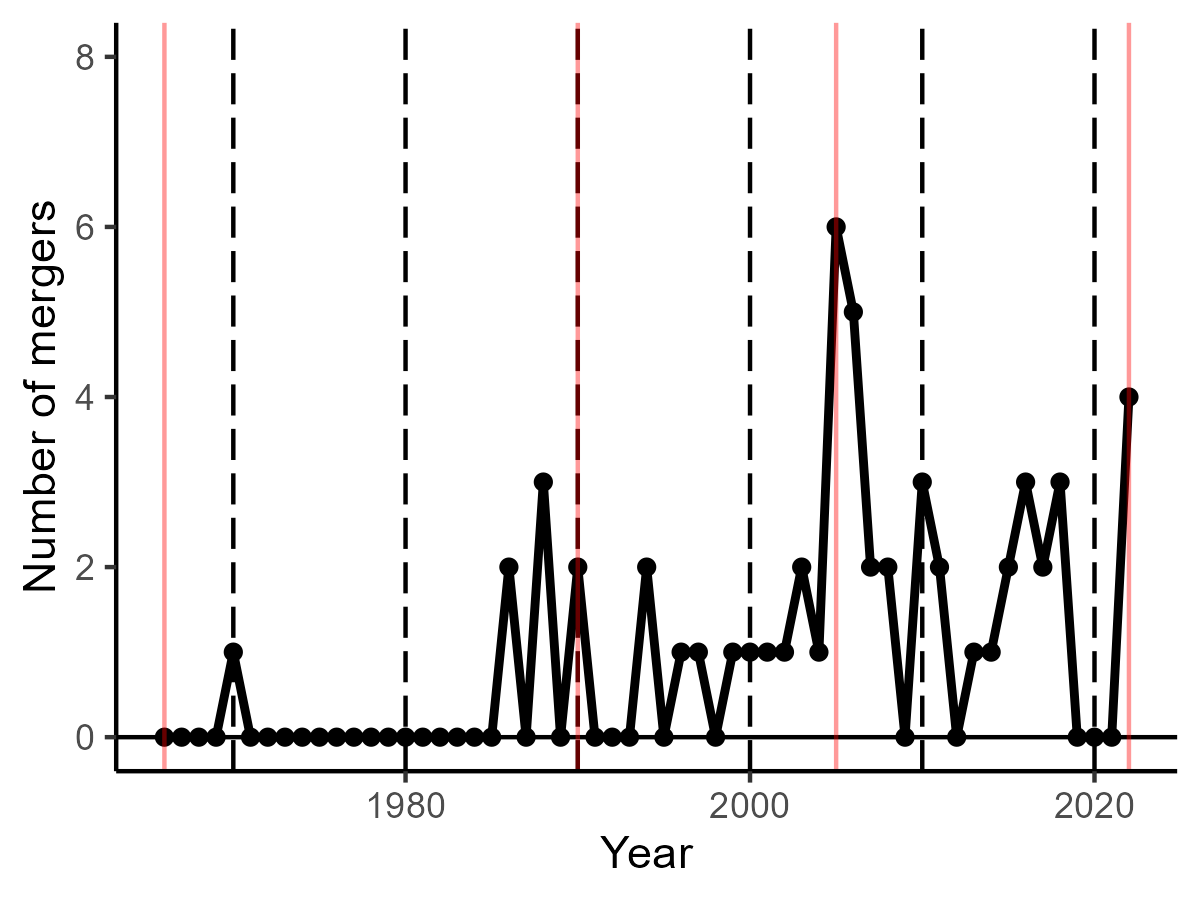
\includegraphics[width = 0.7\textwidth]
  {figuretable/number_of_mergers.png}
  \caption{The number of mergers between 1966 and 2022}
  \label{fg:number_of_mergers}
  \end{center}
\footnotesize
   Note: Red lines divide the regimes based on CIY, IHS, and HB.
\end{figure}

\begin{figure}[!ht]
\begin{center}
  \subfloat[Price]{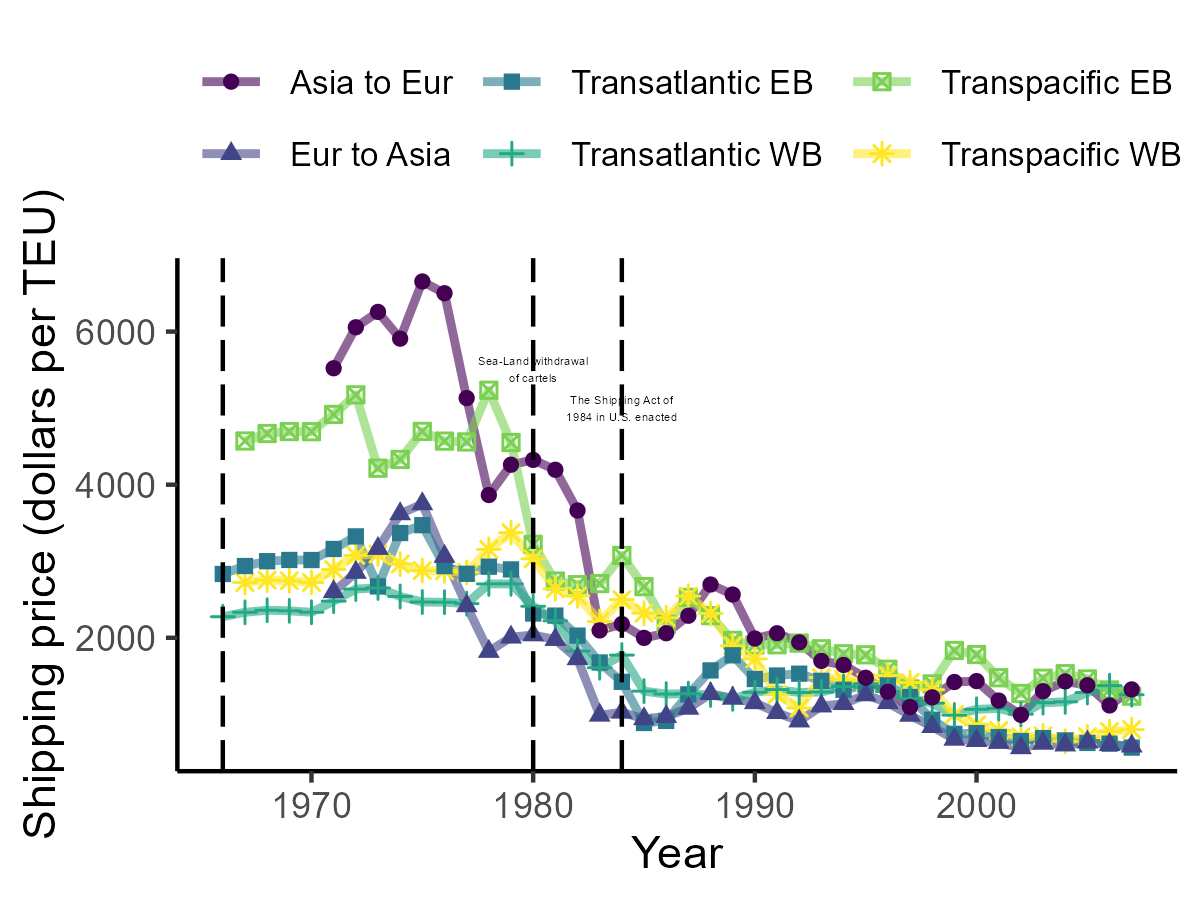
\includegraphics[width = 0.7\textwidth]
  {figuretable/container_freight_rate_each_route.png}}\\
  \subfloat[Quantity]{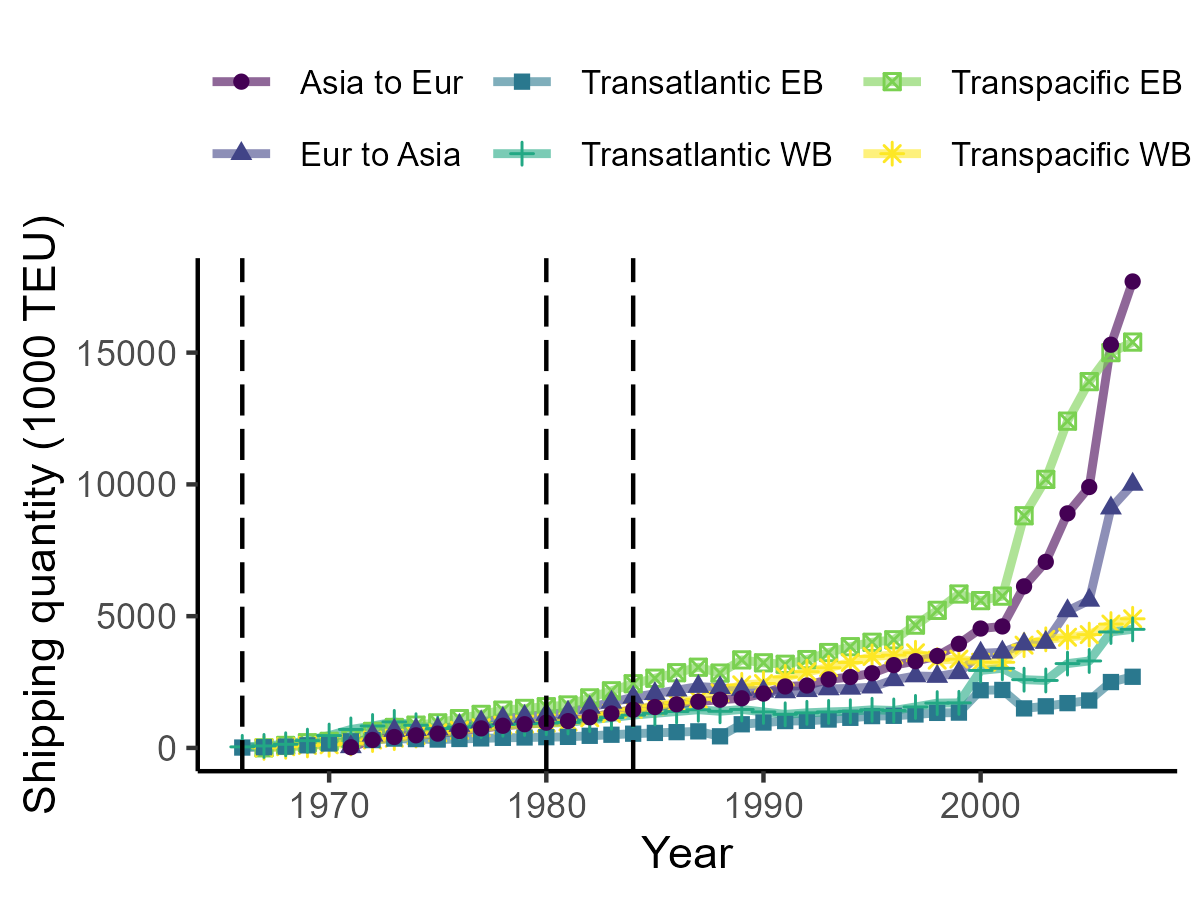
\includegraphics[width = 0.7\textwidth]
  {figuretable/container_shipping_quantity_each_route.png}}
  \caption{Trends in route-year-level shipping prices and quantities.}
  \label{fg:container_freight_rate_and_shipping_quantity_each_route}
  \end{center}
\footnotesize
  Note: Prices are adjusted to the CPI in the U.S. in 1995. See the detail in \cite{matsuda2022unified}.
\end{figure}

\subsection{Industry Background}\label{sec:industry_background}
We describe the industry background between 1966 and 2022 chronologically by focusing on firms' mergers. 
As discussed above, we classify the whole period into three regimes, 1966-1990, 1991-2005, and 2006-2022. Each regime corresponds with the institutional background and data source.
In the following merger lists, we intentionally keep the original names of firms in each regime data although there are inconsistencies across these data.

\begin{table}[!htbp]
  \begin{center}
      \caption{Merger list: CIY (1966-1990)}
      \label{tb:merger_list_CIY} 
      
\begin{tabular}[t]{rllrl}
\toprule
ID & Seller & Buyer & Year & Type\\
\midrule
1 & Moore-McCormack Lines Inc & United States Lines & 1970 & acquisition\\
2 & OCL & P\&O Containers & 1986 & merger\\
3 & Franco-Belgian Services & Maersk & 1986 & merger\\
4 & Y-S Line & NLS & 1988 & merger\\
5 & Japan Line & NLS & 1988 & merger\\
6 & KSC & Hanjin & 1988 & merger\\
7 & Finland Steamship & Finnlines & 1990 & merger\\
8 & Atlanttrafik/Barber Blue Sea & Wilhelmsen Lines A/S & 1990 & merger\\
\bottomrule
\end{tabular}

  \end{center}\footnotesize
  %Note: 
\end{table} 

\begin{table}[!htbp]
  \begin{center}
      \caption{Merger list: IHS (1991-2005)}
      \label{tb:merger_list_IHS} 
      
\begin{tabular}[t]{llr}
\toprule
Seller & Buyer & Year\\
\midrule
IMC SHIPPING CO PTE LTD & IMC SHIPPING CO PTE LTD & 1993\\
BUSAN SHIPPING CO LTD & EUROSEAS LTD & 1994\\
CHINA MERCHANTS STEAM NAVIGATI & China Merchants Group & 1994\\
SVITZER AS & A P MOLLER & 1996\\
APL LTD & NEPTUNE ORIENT LINES LTD (NOL) & 1997\\
PRIMA SHIPMANAGEMENT SDN BHD & HALIM MAZMIN GROUP & 1999\\
FARRELL LINES INC & A P MOLLER & 2000\\
OOST ATLANTIC LIJN BV & ATLANTIC HORIZON GROUP & 2001\\
CYPRUS MARITIME CO LTD & CYPRUS SEA LINES SA & 2002\\
MISC BERHAD & Malaysia Shipping Corp Sdn Bhd & 2003\\
DANSK SUPERMARKED INVEST A/S & A P MOLLER & 2003\\
THE PENINSULAR AND ORIENTAL ST & A P MOLLER & 2004\\
EUROBULK LTD & EUROSEAS LTD & 2005\\
BARCLAY SHIPPING LTD & BARCLAY SHIPPING LTD & 2005\\
DELMAS & CMA CGM HOLDING & 2006\\
ROYAL P\&O NEDLLOYD NV & A P MOLLER & 2006\\
UNITED THAI SHIPPING CORP LTD & IMC SHIPPING CO PTE LTD & 2006\\
HORIZON LINES INC & MATSON NAVIGATION CO INC & 2006\\
EICKE SCHIFFAHRTS KG & EICKE SCHIFFAHRTS KG & 2006\\
CP SHIPS LTD & HAPAG-LLOYD AG & 2006\\
\bottomrule
\end{tabular}

  \end{center}\footnotesize
  %Note: 
\end{table} 

\begin{table}[!htbp]
  \begin{center}
      \caption{Merger list: HB (2006-2022)}
      \label{tb:merger_list_HB} 
      
\begin{tabular}[t]{rllrl}
\toprule
ID & Seller & Buyer & Year & Type\\
\midrule
1 & Cheng Lie & CMA-CGM & 2006 & acquisition\\
2 & Lloyd Triestino & Evergreen & 2006 & merger\\
3 & Norasia & CSAV & 2006 & acquisition\\
4 & MacAndrews & CMA-CGM & 2007 & acquisition\\
5 & Lufeng & Sinotrans & 2008 & merger\\
6 & NEW ONTO SHIPPING & GOTO Shipping International Ltd & 2010 & merger\\
7 & TSK & NYK & 2010 & merger\\
8 & China Navigation & Swire & 2011 & acquisition\\
9 & CCNI & Maersk & 2015 & acquisition\\
10 & CSAV & Hapag-Lloyd & 2015 & acquisition\\
11 & China Shipping & COSCO & 2016 & merger\\
12 & Shanghai Puhai Shipping & COSCO & 2016 & merger\\
13 & UASC & Hapag-Lloyd & 2017 & acquisition\\
14 & KLINE & Ocean Network Express & 2018 & merger\\
15 & MOL & Ocean Network Express & 2018 & merger\\
16 & NYK & Ocean Network Express & 2018 & merger\\
17 & APL & CMA-CGM & 2017 & acquisition\\
18 & Hamburg Sud & Maersk & 2018 & acquisition\\
\bottomrule
\end{tabular}

  \end{center}\footnotesize
  %Note:
\end{table} 

\paragraph{1966-1990} 

Table \ref{tb:merger_list_CIY} summarizes all mergers based on CIY between 1966 and 1990.\footnote{In 1964, the Japanese ocean shipping industry experienced consolidation induced by the government, and 95 firms were merged into six large groups. \cite{otani2021estimating} investigates the event by a structural matching model.}
This period involves a collusive and competitive environment with shipping conferences that are explicit and cartels globally allowed. 
The period is studied in \cite{matsuda2022unified} and \cite{otani2023industry} in detail.
The period is divided into the collusive (1966-1983) and competitive (1984-1990) periods due to the U.S. Shipping Act of 1984.\footnote{The relevant studies are \cite{wilson1991some}, \cite{pirrong1992application}, and \cite{clyde1998market}. \cite{wilson1991some} provided evidence of regime change by the Shipping Act of 1984 using data on quarterly freight rates and shipping quantities of five selected commodities only on the Transpacific route. \cite{pirrong1992application} tested the model prediction of the core theory surveyed in \cite{sjostrom2013competition} using data from two specific trade routes between 1983 and 1985. \cite{clyde1998market} studied the relationship between market power and the market share of shipping conferences after the act. }
In the collusive period between 1966 and 1983, a single merger occurred in 1970 (Moore-McCormack Lines Inc merged by United States Lines). % and 1972 (Johnson Line merged by NA).
In the competitive period between 1984 and 1990, two mergers occurred in 1986, three mergers occurred in 1988, and two mergers occurred in 1990. 
\textcolor{blue}{Anecdotally, mergers in the period are driven by XXX}
% Background
% What mergers?

\paragraph{1991-2008}

Table \ref{tb:merger_list_IHS} summarizes all mergers based on IHS between 1991 and 2005.
The period involves the Ocean Shipping Reform Act (OSRA) of 1998 and this enactment divides the period into the pre-OSRA and post-OSRA periods. 
The period is studied in \cite{fusillo2006some,fusillo2013stability} and \cite{reitzes2002rolling} in detail.
We find that five mergers before 1998 and 17 mergers after 1998 occurred.
\textcolor{blue}{Anecdotally, mergers in the period are driven by XXX}
% Background
% What mergers?




\paragraph{2009-2022}

Table \ref{tb:merger_list_HB} summarizes all mergers based on IHS between 2006 and 2022.
\textcolor{blue}{The period is studied in XXX in detail. Anecdotally, mergers in the period are driven by XXX}
% Background
% What mergers?




% (Need to validate with NYK aggregate TEU data just for confirmation.)

\subsection{Descriptive statistics}\label{sec:descriptive_statistics}

Table \ref{tb:summary_statistics} shows summary statistics of firm-year-level variables of buyer and seller firms in all realized merger cases between 1966 and 2022. 
We construct firm-year-level variables such as the firm's age in the global container shipping industry and size measured by TEU in the merger year. 
We normalize these variables from 0 (minimum age) to 1 (maximum age) in each regime for comparison across regimes.
First, we find that the mean of normalized firms' age decreases from 0.84 in the 1966-1990 period to 0.51 in the 2006-2022 period. 
This implies that mergers are likely to occur between relatively younger firms in recent years.
Second, the mean of normalized firms' size decreases from 0.23 in the 1966-1990 period to 0.08 in the 2006-2022 period. 
This implies that mergers are likely to occur between relatively smaller firms in recent years, although the firm's absolute size increases exponentially, in particular, between 2006 and 2022. 
Note that we treat new entrant firms buying incumbent firms as firms whose age and size are zero so that the above findings capture that the number of entries by mergers increases.
Figure \ref{fg:size_cdf} illustrates the cumulative distributions of the normalized firm's size and age for each regime. 
This confirms the above fact that mergers are likely to involve relatively younger and smaller firms in recent years.


\begin{table}[!htbp]
  \begin{center}
      \caption{Summary statistics of firm-year-level variables}
      \label{tb:summary_statistics} 
      \subfloat[CIY (1966-1990)]{
\begin{tabular}[t]{lrrrrr}
\toprule
  & N & mean & sd & min & max\\
\midrule
Age (Normalized) & 16 & 0.84 & 0.24 & 0.23 & 1.00\\
Size TEU (Normalized) & 16 & 0.23 & 0.29 & 0.01 & 1.00\\
\bottomrule
\end{tabular}
}\\
      \subfloat[IHS (1991-2005)]{
\begin{tabular}[t]{lrrrrr}
\toprule
  & N & mean & sd & min & max\\
\midrule
Age (Normalized) & 40 & 0.58 & 0.39 & 0.00 & 1.00\\
Size TEU (Normalized) & 40 & 0.11 & 0.22 & 0.00 & 1.00\\
\bottomrule
\end{tabular}
}\\
      \subfloat[HB (2006-2022)]{
\begin{tabular}[t]{lrrrrr}
\toprule
  & N & mean & sd & min & max\\
\midrule
Age (Normalized) & 60 & 0.51 & 0.30 & 0.11 & 1.00\\
Size TEU (Normalized) & 60 & 0.08 & 0.19 & 0.00 & 1.00\\
\bottomrule
\end{tabular}
}
      
  \end{center}\footnotesize
  %Note:
\end{table} 

\begin{figure}[!ht]
\begin{center}
  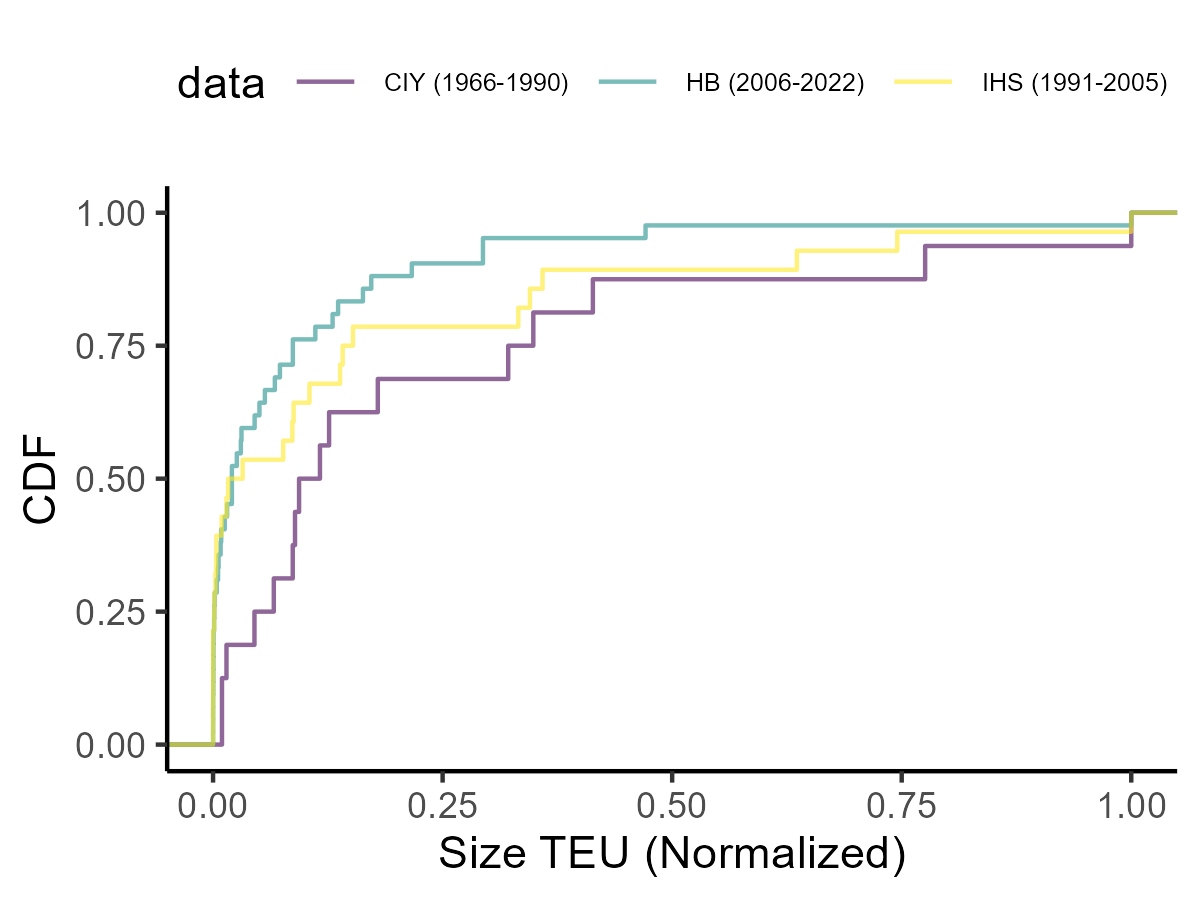
\includegraphics[width = 0.45\textwidth]
  {figuretable/normalized_size_cdf.png}
  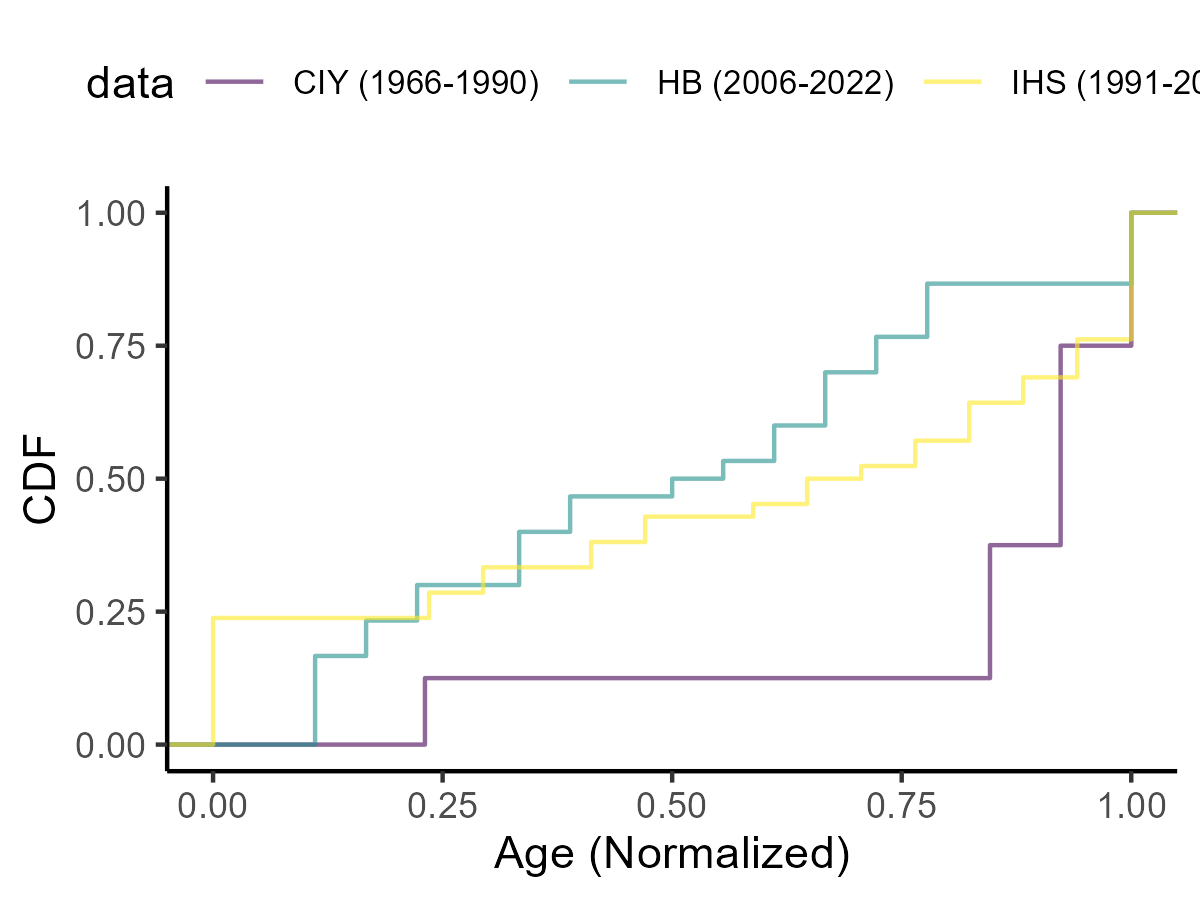
\includegraphics[width = 0.45\textwidth]
  {figuretable/normalized_age_cdf.png}
  \caption{Distributions of firm-year-level variables for each regime}
  \label{fg:size_cdf}
  \end{center}
\footnotesize
   %Note: 
\end{figure}

\begin{figure}[!ht]
\begin{center}
  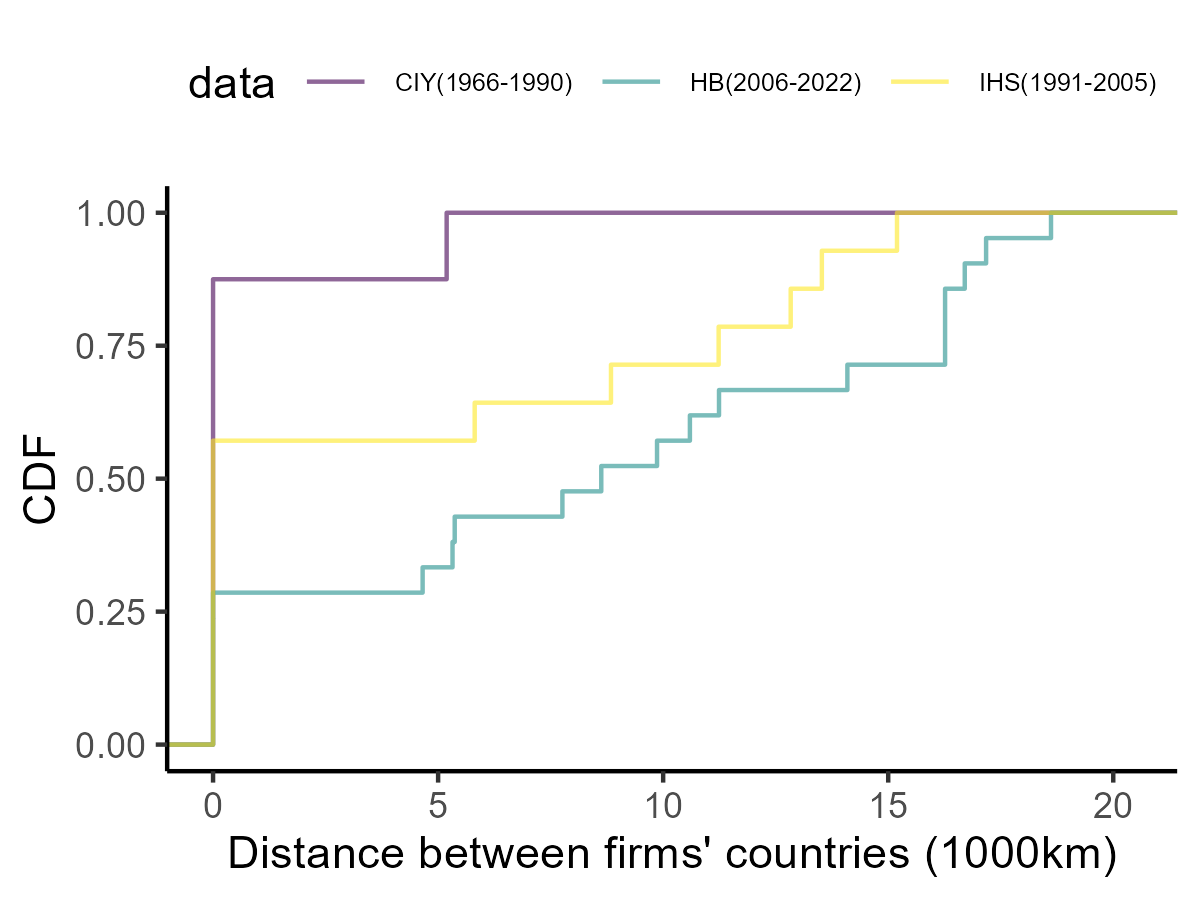
\includegraphics[width = 0.7\textwidth]
  {figuretable/distance_cdf.png}
  \caption{Distributions of match-level distances of seller and buyer firms for each regime}
  \label{fg:distance_cdf}
  \end{center}
\footnotesize
   %Note: 
\end{figure}


Figure \ref{fg:distance_cdf} illustrates distributions of realized match-level distances. 
We find that almost all mergers between 1966 and 1990 involve buyer and seller firms in the same country. 
Although the share of mergers in the same country is more than 40 \% in the whole period, the share of mergers of firms between countries separated by distance increases in recent years. 
This implies that the reason why mergers occur might change from domestic one to global one due to the prosperity and expansion of international container transport.

These tables and figures provide some intuition that mergers are likely to involve relatively younger and smaller firms in more distant countries in recent years. 
However, disentangling the relative importance of each variable with limited data needs a more sophisticated structural model.
In Section \ref{sec:empirical_analysis}, we construct a structural matching model to quantify the relative importance of each variable and compare the transition across regimes.




\section{Empirical analysis}\label{sec:empirical_analysis}

Our objective is to quantify the assortativeness of observed characteristics for each regime and compare the levels across regimes. 
We employ a matching maximum score estimator developed by \cite{fox2018qe}, which is one of the most well-known methods for measuring matching assortativeness.

For exposition, we model mergers in each regime as a two-sided one-to-one transferable matching game in a single market. Let $\mathcal{N}_b$ and $\mathcal{N}_s$ be the sets of potential finite buyers and sellers respectively. Let $b=1,\cdots,|\mathcal{N}_b|$ be buyer firms and let $s=1,\cdots,|\mathcal{N}_s|$ be seller firms where $|\cdot|$ is cardinality. Let $\mathcal{N}_{b}^{m}$ denote the set of ex-post matched buyers and $\mathcal{N}_{b}^{u}$ denote that of ex-post unmatched buyers such that $\mathcal{N}_b= \mathcal{N}_{b}^{m}\cup\mathcal{N}_{b}^{u}$ and $\mathcal{N}_{b}^{m}\cap\mathcal{N}_{b}^{u}=\emptyset$. For the seller side, define $\mathcal{N}_{s}^{u}$ and $\mathcal{N}_{s}^{m}$ as the set of ex-post matched and unmatched sellers such that $\mathcal{N}_s= \mathcal{N}_{s}^{m}\cup\mathcal{N}_{s}^{u}$ and $\mathcal{N}_{s}^{m}\cap\mathcal{N}_{s}^{u}=\emptyset$. Let $\mathcal{M}^m$ be the sets of all ex-post matched pairs $(b,s)\in\mathcal{N}_{b}^{m}\times \mathcal{N}_{s}^{m}$. Let $\mathcal{M}$ denote the set of all ex-post matched pairs $(b,s)\in\mathcal{M}^{m}$ and unmatched pairs $(\tilde{b},\emptyset)$ and $(\emptyset,\tilde{s})$ for all $\tilde{b}\in \mathcal{N}_b^u$ and $\tilde{s}\in \mathcal{N}_s^u$ where $\emptyset$ means a null agent generating unmatched payoff. 

Each firm can match at most one agent on the other side, so  $|\mathcal{N}_b^{m}|=|\mathcal{N}_s^{m}|$. The matching joint production function is defined as $f(b,s)=V_b(b,s)+V_s(b,s)$ where $V_b:\mathcal{M}\rightarrow \mathbb{R}$ and $V_s:\mathcal{M}\rightarrow \mathbb{R}$. The net matching values for buyer $b$ and seller $s$ are defined as $V_b(b,s)=f(b,s)-p_{b,s}$ and $V_s(b,s)+p_{b,s}$, where $p_{b,s}\in \mathbb{R}_{+}$ is the equilibrium merger price paid to seller firm $s$ by buyer firm $b$ and $p_{b\emptyset}=p_{\emptyset s}=0$. For scale normalization, we assume $V_b(b,\emptyset)=0$ and $V_s(\emptyset,s)=0$ for all $b\in \mathcal{N}_b$ and $s\in \mathcal{N}_s$. Each buyer maximizes $V_b(b,s)$ across seller firms, whereas each seller maximizes $V_s(b,s)$ across buyer firms. 

The stability conditions for buyer firm $b \in \mathcal{N}_b$ and seller firm $s \in \mathcal{N}_s$ are as follows:
\begin{align}
    V_b(b,s) &\ge V_b(b,s') \quad \forall s' \in \mathcal{N}_s \cup \emptyset,s'\neq s,\label{eq:stability_ineq}\\
    V_s(b,s) &\ge V_s(b',s) \quad \forall b' \in \mathcal{N}_b\cup \emptyset,b'\neq b.\nonumber
\end{align}

Based on Inequalities \eqref{eq:stability_ineq} and equilibrium price conditions $p_{b',s}\le p_{b,s}$ and $p_{b,s'}\le p_{b',s'}$ in \cite{akkus2015ms}, we construct the inequalities for matches $(b,s)\in \mathcal{M}$ and $(b',s')\in \mathcal{M}, (b',s')\neq(b,s)$ as follows:
\begin{align}
    f(b,s)-f(b,s')&\ge p_{b,s}-p_{b,s'}\ge p_{b,s}-p_{b',s'},\label{eq:pairwise_stable_ineq}\\
    f(b',s')-f(b',s)&\ge p_{b',s'}-p_{b',s}\ge p_{b',s'}-p_{b,s},\nonumber\\
    V_s(b,s)-V_s(b',s)&\ge 0,\nonumber\\
    V_{s'}(b',s')-V_s(b,s')&\ge 0,\nonumber
\end{align}
where $p_{b',s}$ and $p_{b,s'}$ are unrealized equilibrium merger prices that cannot be observed in the data. The last two inequalities cannot be derived from the data because the researchers cannot observe how the total matching value $f(b,s)$ is shared between buyer $b$ and seller $s$.

Each buyer firm can only acquire one seller firm, which implies that the buyer firm’s
choice among a set of seller firms is a discrete choice. 
As a simple semiparametric technique to estimate this discrete choice, we turn to maximum score estimation \cite{manski1975maximum,manski1985semiparametric}.
\cite{fox2018qe} proposes a maximum score
estimator using the above inequalities when we observe the transfer data or not under mild conditions. 
The maximum score estimator is consistent if the model satisfies a rank order property as in \cite{manski1975maximum,manski1985semiparametric}, i.e., the probability of observing matched pairs is larger than the probability of observing swapped matched pairs. 
The rank order property is equivalent to pairwise stability which is a milder property rather than stability, so that the rank order property holds under the above stability conditions. See identification details in \cite{fox2010qe} and Monte Carlo simulation results in \cite{fox2018qe}, \cite{akkus2015ms}, and \cite{otani2021matching_cost}.

We specify $f(b,s)$ as a parametric form $f(b,s|X,\beta)$ where $X$ is a vector of observed characteristics of all buyers and sellers and $\beta$ is a vector of parameters. 
In the absence of transfer data, given the observed characteristics $X$, one can estimate $\beta$ by maximizing the following objective function:
\begin{align}
    Q(\beta)=\sum_{(b,s)\in \mathcal{M}} \sum_{(b',s')\in \mathcal{M},(b',s')\neq (b,s)} \mathbbm{1}[f(b,s|X,\beta)+ f(b',s'|X,\beta)\ge f(b,s'|X,\beta)+f(b',s|X,\beta)]\label{eq:score_function}
\end{align}
where $\mathbbm{1}[\cdot]$ is an indicator function. 
The inequality is constructed by adding the first two inequalities and canceling out transfers $p_{b,s}$ and $p_{b',s'}$ in Inequalities \eqref{eq:pairwise_stable_ineq}.
The objective function \eqref{eq:score_function} counts the number of correctly predicted pairwise stable matching under each candidate parameter $\beta$.


In our empirical application, as the observed characteristics, $X$, we use the standardized firm's age, size measured by the total tonnage, and match-level distance calculated from the locations of the flag countries at merger timing, that is, all observed variables are standardized to $[1e-6,1]$. 
Concretely, we specify the joint production function $f(b,s)$ as
\begin{align}
    f(b,s|X,\beta)= \beta_1 \text{Age}_{b}\text{Age}_{s} + \beta_2 \text{Size}_{b}\text{Size}_{s} + \beta_3 \text{Distance}_{bs} + \varepsilon_{bs},\label{eq:joint_production}
\end{align}
where $\varepsilon_{bs}$ is assumed to be i.i.d. errors drawn from the zero median distribution as in \cite{fox2018qe}. 
Note that any parameters of firm-specific characteristics cannot be identified with maximum score estimation based solely on without-transfers information. With transfer data, $p_{b,s}$ and $p_{b',s'}$, such as the payments regarding mergers from buyer firms to seller firms, the identification is possible and the precision of the estimator improves as in \cite{akkus2015ms}.


\section{Results}\label{sec:results}

Table \ref{tb:maximum_score_estimate} reports the estimation results of the matching maximum score estimator. 
Since we can use only realized merger cases, we could not construct a 95 \% confidence interval with enough subsampled data via bootstrap.
Instead, the numbers in brackets indicate the lower and upper bounds of a set of maximizers of the objective function. 
If the lower and upper bounds are the same, then the parameters are point-identified. 
Otherwise, the parameters are partially identified.
The percent of correct matches used as a measure of statistical fit is more than 90\%, so the estimated model predicts the actual mergers well.

First, the estimated coefficient of the firm's size shows an interesting transition. 
The sign is changed from ambiguous between 1966 and 1990, positive between 1991 and 2005, to negative between 2006 and 2022. 
In particular, between 1991 and 2005, as a positive factor, a firm's size is more important than a firm's age by seven to nine times in merger decisions, that is, a firm's size works as a merger incentive.
On the other hand, between 2006 and 2022, as a negative factor, a firm's size is more important than a firm's age by 1.4 times, that is, a firm's size works as a merger disincentive.
\textcolor{blue}{These results are consistent with the institutional fact that XXX}

Second, the estimated coefficient of the distance of seller and buyer firms shows a negative sign across all regimes but the level decreases between 2006 and 2022. 
This means that mergers of firms in distant countries are likely to occur, but the importance level relative to a firm's age has decreased to economically zero in recent years.
\textcolor{blue}{These results are consistent with the institutional fact that XXX}

\begin{table}[!htbp]
  \begin{center}
      \caption{Matching maximum score estimation}
      \label{tb:maximum_score_estimate} 
      
\begin{tabular}[t]{lcc}
\toprule
Regime & 1966-1990 & 2005-2022\\
Standardized Firm age & 1 & 1\\
Standardized Firm-year-level TEU & {}[3e-04,0.0331] & {}[0.0019,0.1197]\\
\% of correct matches & 0.9643 & 0.9715\\
\bottomrule
\end{tabular}

  \end{center}\footnotesize
  Note: The objective function was numerically maximized using differential evolution (DE) algorithm in \texttt{BlackBoxOptim.jl} package. For DE algorithm, we require setting the domain of parameters and the number of population seeds so that we fix the former to $[-10, 10]$. For estimation, 100 runs of 1,000 seeds were performed for all specifications. The numbers in parentheses are the lower and upper bounds of the set of maximizers of the maximum rank estimator. Parameters that can take on only a finite number of values (here 1) converge at an arbitrarily fast rate, then they are superconsistent. The unit of measure of all variables is normalized to $[1e-6,1]$. 
\end{table} 

\section{Counterfactual}\label{sec:counterfactuals}

In the global container shipping industry, mergers between firms in the same country involve several concerns from competition policies in multiple countries.
For example, on June 21, 2017, South Africa's Competition Commission issued a statement stating that it "forbade" the integration of the container business by the three shipping lines of NYK, MOL, and KLINE. 
The commission cited concerns about market consolidation by domestic companies and cartel issues involving these companies in the car carrier business.
The country's competition court finally approved the integration on January 17, 2018, but this could impact the planned launch of the integrated container company, Ocean Network Express. 
\textcolor{blue}{[Other example?]}

In our counterfactual simulation, given estimated parameters, we simulate the matching outcome under the hypothetical scenario that mergers between firms in the same country are prohibited. 
Mechanically, first, this scenario uses the merger cases of firms in different countries and imposes that 
the joint production function \eqref{eq:joint_production} is changed to
\begin{align*}
    f(b,s|X,\beta)= \begin{cases}
        \beta_1 \text{Age}_{b}\text{Age}_{s} + \beta_2 \text{Size}_{b}\text{Size}_{s} + \beta_3 \text{Distance}_{bs} + \varepsilon_{bs}, \quad \text{if }\text{Distance}_{bs}\neq 1e-6,\\
        -\infty, \quad \text{otherwise}.
    \end{cases}
\end{align*}
Second, given counterfactual $f(b,s|X,\beta)$, we compute an equilibrium matching allocation. 
The equilibrium one-to-one matching allocation $\{m(b,s)\}_{b\in\mathcal{N}_b,s\in\mathcal{N}_s}$ is calculated by the following linear programming problem proposed by \cite{shapley1971assignment}:
\begin{align*}
    \max_{\{m(b,s)\}_{b\in\mathcal{N}_b,s\in\mathcal{N}_s}} &f(b,s|X,\beta)\cdot m(b,s),\\
    \text{s.t. } 0&\le \sum_{b\in\mathcal{N}_b}m(b,s)\le 1\quad  \forall s \in \mathcal{N}_s,\\
    0&\le \sum_{s\in\mathcal{N}_s}m(b,s)\le 1\quad \forall b \in \mathcal{N}_b,\\
    0&\le m(b,s) \quad \forall b \in \mathcal{N}_b,\forall s \in \mathcal{N}_s
\end{align*}
where the dual of this linear programming problem also gives equilibrium prices. 
We allow firms to be unmatched to avoid gaining negative joint production functions.
In the simulation, we fix the parameters to the upper bounds of estimated parameters in Table \ref{tb:maximum_score_estimate}, and we draw 100 i.i.d. draws of $\varepsilon_{bs}$ from the standard normal distribution $N(0,1)$, then solve the above linear programming problem.
We confirm that using the lower bounds of parameters gives almost the same results.
We report the most frequently observed matching outcomes.

\begin{table}[!htbp]
  \begin{center}
      \caption{Counterfactual simulations under the prohibition of mergers of firms in the same country}
      \label{tb:number_of_mergers_counterfactual} 
      
\begin{tabular}[t]{lccc}
\toprule
Regime &  & 1991-2005 & 2006-2022\\
\midrule
\% total match (counterfactual/data) &  & 0.714 & 1.000\\
\% same match (counterfactual/data) &  & 0.222 & 0.222\\
Matching Num (data) &  & 7 & 18\\
\bottomrule
\end{tabular}

  \end{center}\footnotesize
  %Note: 
\end{table} 

Table \ref{tb:number_of_mergers_counterfactual} reports the counterfactual simulation results under the prohibition of mergers between firms in the same country. 
Since only one merger of firms in different countries happened between 1966 and 1990, we focus on the periods between 1991 and 2005, and between 2006 and 20022.
First, between 1991 and 2005, the number of mergers between firms in different countries decreases by 28.6\% in the counterfactual scenario because XXX. 
Also, 22.2\% of the counterfactual merger pairs are the same as actual pairs.
This implies that XXX.
Second, between 2006 and 20022, the number of mergers between firms in different countries is the same as the data. 
Also, 22.2\% of the counterfactual merger pairs are the same as actual pairs. 
This implies that XXX.

Therefore, we find that the prohibition of mergers between firms in the same country affects not only the number of permitted mergers in different countries but also the merger configuration, that is, buyer-seller-match pairs.




\section{Interviews}\label{sec:interviews}

\textcolor{blue}{Concerning the transition of merger incentives from 1966 to 2022, Mr.
Akimitsu Ashida, former chairman of Mitsui O.S.K. Lines (MOL), answered about the situation in those days. He served as the company’s European Division Manager from 1985-86 and responded
to our e-mail inquiry on XXX. We asked him about his thoughts and related memory on the figures, tables, and our results.}



\section{Practical Implications, Discussion, and Future Research}\label{sec:practical_implications}

\subsection{Practical Implications}

Our study makes an important contribution to the development of the unified merger list of the container shipping industry and policy discussions for practitioners. 
The data contribution enables practitioners to obtain empirical and historical knowledge on the main container transport markets, as well as to develop a methodology to disentangle merger incentives.
\textcolor{blue}{For example, XXX.} Also, \cite{jeon2022learning} simulates counterfactual merger scenarios of specific two firms between 2006 and 2014 but does not incorporate and explain other more than ten merger cases in her model.
Thus, our data contribution complements previous studies institutionally and sheds light on the date patterns and main drivers of mergers in the industry.


\subsection{Discussion}
We summarize the potential concerns for the data and methodology. 
First, we merge three data sources that record potentially different variables and observations for each regime. 
Thus, we could not check the robustness check on the choice of regime, although we believe that our choice of regime is reasonable for institutional and graphical reasons.
Second, we may face a small sample problem, in particular, between 1966 and 1990 even though the matching maximum score approach works in a small sample in Monte Carlo simulations \citep{akkus2015ms,otani2021matching_cost}.
Third, we drop merger cases that involve firms whose variables are missing in our three data sources. 
\textcolor{blue}{This might be because XXX.}


\subsection{Future Research}

We should discuss possible extensions as well as some shortcomings of this study. 
As a methodological issue, first, this paper focuses on disentangling endogenous merger incentives while ignoring future competition in the market due to data limitations. 
Thus, a welfare evaluation of the post-merger market was not investigated.
Combining firms' strategic interactions with estimations of demand and supply sides with the endogenous matching merger model remains a challenging and open research question in the field of industrial organization \citep{agarwal2021market}. 
An exceptional study is \cite{igami2019mergers} which construct a stochastic sequential-move game but need monthly-level merger data and allow only a single merger each month. 
Developing their approach might resolve the relationship between matching and competition.
Second, our matching model does not incorporate unobserved heterogeneity which is identified nonparametrically \citep{fox2018jpe}.
Pursuing this direction will require a different econometric approach such as the simulated method of moments in \cite{fox2018jpe} and multiple market data. 

\textcolor{blue}{As an institutional and data issue, first, XXX}



\section{Conclusion}\label{sec:conclusion}
We construct a novel unified list of mergers in the global container shipping industry between 1966 (the beginning of the industry) and 2022. 
Combining the list with proprietary data, we construct a structural matching model \citep{fox2018qe} to describe the historical transition of the importance of a firm's age, size, and geographical proximity on merger decisions. 
We find different transition patterns of the importance of a firm's age, size, and geographical proximity.
In counterfactual simulations, we find that the prohibition of mergers between firms in the same country affects not only the number of permitted mergers in different countries but also the merger configuration, that is, buyer-seller-match pairs.

\textbf{Acknowledgement} \\
\textcolor{blue}{We benefited from anonymous referees and participants at the XXX. We thank Akimitsu Ashida and Hiroyuki Sato for sharing industry knowledge and expertise as ex-chairperson in the 1980s and Jeremy Fox for introducing methodology. And we thank Mikio Tasaka, Yasuhiro Fujita, Jong-khil Han and Yutaka Yamomoto for professional comments. This study was supported by JSPS KAKENHI Grant Numbers 20K22129 and 22K13501. }



\bibliographystyle{aer}
\bibliography{container_merger_data_bib}


\end{document}